\documentclass[a4paper,12pt]{article} % тип документа

% Поля страниц
\usepackage[left=2.5cm,right=2.5cm,
    top=2cm,bottom=2cm,bindingoffset=0cm]{geometry}
    
%Пакет дял таблиц   
\usepackage{multirow} 
    
%Отступ после заголовка    
\usepackage{indentfirst}


% Рисунки
\usepackage{floatrow,graphicx,calc}
\usepackage{wrapfig}

%%% Работа с картинками
\usepackage{graphicx}  % Для вставки рисунков
\graphicspath{{images/}}  % папки с картинками
\setlength\fboxsep{3pt} % Отступ рамки \fbox{} от рисунка
\setlength\fboxrule{1pt} % Толщина линий рамки \fbox{}
\usepackage{wrapfig} % Обтекание рисунков и таблиц текстом

% Создаём новый разделитель
\DeclareFloatSeparators{mysep}{\hspace{1cm}}

% Ссылки?
\usepackage{hyperref}
\usepackage[rgb]{xcolor}
\hypersetup{				% Гиперссылки
    colorlinks=true,       	% false: ссылки в рамках
	urlcolor=blue          % на URL
}


%  Русский язык
\usepackage[T2A]{fontenc}			% кодировка
\usepackage[utf8]{inputenc}			% кодировка исходного текста
\usepackage[english,russian]{babel}	% локализация и переносы

% Математика
\usepackage{amsmath,amsfonts,amssymb,amsthm,mathtools}

%%% Дополнительная работа с математикой
\usepackage{amsmath,amsfonts,amssymb,amsthm,mathtools} % AMS
\usepackage{icomma} % "Умная" запятая: $0,2$ --- число, $0, 2$ --- перечисление

% Что-то 
\usepackage{wasysym}


\begin{document}
\begin{center}
	\footnotesize{ФЕДЕРАЛЬНОЕ ГОСУДАРСТВЕННОЕ АВТОНОМНОЕ ОБРАЗОВАТЕЛЬНОЕ 			УЧРЕЖДЕНИЕ ВЫСШЕГО ОБРАЗОВАНИЯ}\\
	\footnotesize{МОСКОВСКИЙ ФИЗИКО-ТЕХНИЧЕСКИЙ ИНСТИТУТ\\(НАЦИОНАЛЬНЫЙ 			ИССЛЕДОВАТЕЛЬСКИЙ УНИВЕРСИТЕТ)}\\
	\footnotesize{ФИЗТЕХ-ШКОЛА ФИЗИКИ И ИССЛЕДОВАНИЙ им. ЛАНДАУ\\}
	\hfill \break
	\hfill \break
	\hfill \break
	\hfill \break
\end{center}

\begin{center}   
    \hfill \break
	\hfill \break
	\hfill \break
	\hfill \break    \hfill \break
	\hfill \break
	\hfill \break
	\hfill \break
    \hfill \break
    \hfill \break
	\hfill \break
	\large{Лабораторная работа № 2.2.3\\\textbf{Измерение теплопроводности воздуха при атмосферном давлении}}\\
	\begin{flushright}
		Плотникова Анастасия Александровна\\
		Группа Б02-406
	\end{flushright}
	\hfill \break
	\hfill \break
	\hfill \break
\end{center}
\hfill \break
\hfill \break
\hfill \break
\hfill \break
\hfill \break
\hfill \break
\hfill \break
\hfill \break
\hfill \break
\hfill \break
\hfill \break
\hfill \break
\hfill \break
\begin{center}
	Долгопрудный, 2025 г.
\end{center}
\thispagestyle{empty}
\newpage
	\textbf{Цель работы:}\\ 
  измерить коэффициент теплопроводности воздуха при атмосферном
давлении в зависимости от температуры
	\hfill \break
	
	\textbf{В работе используются:}\\ 
  цилиндрическая колба с натянутой по оси платиновой нитью; \\
  термостат Witeg WCR-22 (поддержание: $\pm 0.1 ,\ K$); \\
  вольтметр B7-78/1: 
  \par $\pm (0.009U + 0.001)/100$ В в диапазоне 1 В; 
  \par $\pm (0.012U + 0.002)/100$ В в диапазоне 10 В; \\
  амперметр B7-78/3: 
  \par $\pm (0.05 I + 1)/100$ мА в диапазоне 100 мА; \\
  эталонное сопротивление; \\
  источник постоянного напряжения; \\
  магазин сопротивлений.

\section*{Теоретическая справка}

\textbf{Теплопроводность} — это процесс передачи тепловой энергии от нагретых частей системы к холодным за счёт хаотического движения частиц среды. 

\textbf{Закон Фурье}. Плотность потока энергии $\vec{q}$ (Вт/м$^2$) — количество теплоты, переносимое через единичную площадку в единицу времени — пропорциональна градиенту температуры $\nabla T$:
\begin{equation}
    \vec{q} = -\kappa \cdot \nabla T, \label{eq:fourier}
\end{equation}
где $\kappa$ (Вт/(м$\cdot$К)) — коэффициент теплопроводности.

Оценка для коэффициента теплопроводности газов:
\begin{equation}
    \kappa \sim \lambda \bar{v} \cdot n c_V, \label{eq:kappa_estimate}
\end{equation}
где:\\ 
$\lambda$ — длина свободного пробега молекул газа,\\
$\bar{v} = \sqrt{\dfrac{8k_B T}{\pi m}}$ — средняя скорость теплового движения молекул, \\
$n$ — концентрация (объёмная плотность) газа, \\
$c_V = \dfrac{i}{2}k_B$ — теплоёмкость при постоянном объёме на одну молекулу, \\
$i$ — эффективное число степеней свободы молекулы. \\

Формула \eqref{eq:kappa_estimate} даёт лишь оценку по порядку величины и правильную функциональную зависимость. В учебной литературе часто приводится формула с численным коэффициентом $\frac{1}{3}$. Но это не более, чем оценка. 
\[
    \kappa = \frac{1}{3} \lambda \bar{v} \cdot n c_V.
\]

Длина свободного пробега может быть оценена как $\lambda = \dfrac{1}{n \sigma}$, где $\sigma$ — эффективное сечение столкновений молекул друг с другом.

Тогда из \eqref{eq:kappa_estimate} видно, что коэффициент теплопроводности газа не зависит от плотности газа и определяется только его температурой. В простейшей модели твёрдых шариков $\sigma = \text{const}$, и коэффициент теплопроводности пропорционален корню из абсолютной температуры:
\[
    \kappa \propto \frac{\bar{v}}{n} \propto \sqrt{T}.
\]

На практике эффективное сечение $\sigma(T)$ следует считать медленно убывающей функцией $T$, поскольку при увеличении $T$ молекулы движутся быстрее и проводят меньше времени во интенсивном взаимном взаимодействии, что снижает вероятность эффективного столкновения.

\medskip

Рассмотрим стационарную теплопередачу от тонкой нити (радиус $r_1$, длина $L$), расположенной вдоль оси цилиндра (радиус $r_0$), к его стенкам с постоянной температурой $T_0$. В нити выделяется мощность $Q$. При $L \gg r_0$ теплоотвод через торцы пренебрежимо мал, поток тепла направлен радиально, параметры зависят только от $r$.

Скалярная форма закона Фурье:
\begin{equation}
    q = -\kappa \frac{dT}{dr}.
\end{equation}

Полный поток через цилиндрическую поверхность:
\begin{equation}
    Q = -2\pi r L \cdot \kappa \frac{dT}{dr} = \text{const}.
\end{equation}

При малом перепаде температур $\Delta T = T_1 - T_0$ и $\kappa \approx \kappa(T_0)$, интегрирование даёт:
\begin{equation}
    Q = \frac{2\pi L \kappa \Delta T}{\ln(r_0 / r_1)}
    \label{Q}
\end{equation}

Видно, что закон Ньютона выполняется, то есть поток тепла через систему пропорционален разности температур в
ней.

\subsection*{Оценка времени установления равновесия}

При изменении температуры или мощности нагрева система переходит в новое стационарное состояние за конечное время~$\tau$. Оценим его по порядку величины для плоского слоя толщиной~$a$ и площадью~$S$, заполненного газом при постоянном давлении. 

Температурный скачок~$\Delta T$ вызывает тепловой поток:
\[
q \sim \kappa \frac{\Delta T}{a}.
\]

Для нагрева слоя на~$\Delta T$ требуется тепло:
\[
Q_\text{необх.} = n S a \cdot c_P \Delta T.
\]

Поступившее за время~$\tau$ тепло:
\[
Q = q S \tau = \kappa \frac{\Delta T}{a} S \tau.
\]

Приравнивая, получаем оценку:
\[
\tau \sim \frac{a^2}{\chi}, \quad \text{где} \quad \chi = \frac{\kappa}{n c_P}.
\]
Величина~$\chi$ — температуропроводность, определяет скорость теплового выравнивания. Для воздуха при Н.У. $\chi \sim 0{,}2~\text{см}^2/\text{с}$, при $a \sim 1~\text{см}$ получаем~$\tau \sim 5~\text{с}$.

\subsection*{Пределы применимости теории}

Закон Фурье может нарушаться, если характерные размеры задачи сравнимы с длиной свободного пробега~$\lambda$. Тогда возникает, например, температурный скачок между нитью и газом. В данной работе этим можно пренебречь, так как при атмосферном давлении:
\[
\lambda \sim 10^{-5}~\text{см} \ll r_\text{нити}.
\]

Также возможны и другие механизмы теплопередачи: конвекция и излучение.

\textbf{Конвекция:} подавляется вертикальной ориентацией установки (градиент температуры горизонтален).

\textbf{Излучение:} становится заметным при сильном перегреве нити. Мощность излучения по закону Стефана–Больцмана:
\[
Q_{\text{изл}} = \epsilon \sigma_S S (T_1^4 - T_0^4) \approx 4 \epsilon \sigma_S S T_0^3 \Delta T,
\]
где $\sigma_S = 5{,}67 \cdot 10^{-8}~\text{Вт}/(\text{м}^2\cdot\text{К}^4)$, $\epsilon \sim 0{,}1 \div 0{,}2$ — коэффициент черноты для полированных металлов. В условиях опыта вклад излучения мал.



\section*{Экспериментальная установка}

Схема установки изображена на рисунке (\ref{fig:setup}). 

\begin{figure}[h!]
  \centering
  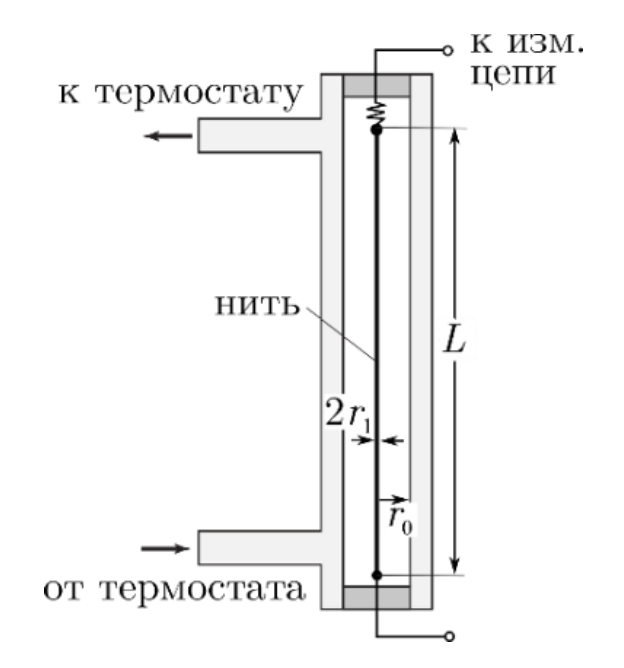
\includegraphics[scale = 0.5]{setup.png}
  \caption{Схема установки}
  \label{fig:setup}
\end{figure}

Внутри вертикально расположенной полой цилиндрической трубки диаметром $2r_0 \sim 1$ см размещена металлическая нить диаметром $2r_1 \sim 0{,}05$ мм и длиной $L \sim 40$ см. Трубка заполнена воздухом и соединена с атмосферой. Стенки охлаждаются водой из термостата, поддерживающего температуру $t_0$. Вертикальное расположение исключает конвекцию.

Нить служит источником тепла и термометром сопротивления. По закону Джоуля–Ленца:
\[
Q = UI, \qquad R = \frac{U}{I}.
\]

Сопротивление $R(t)$ однозначно связано с температурой. При $Q \to 0$ температура нити $t_1 \to t_0$, что позволяет определить зависимость $R(t)$. Альтернативно, используется табличная зависимость удельного сопротивления от температуры.

Относительное изменение сопротивления при $\Delta t = 1^\circ$C обычно составляет $0.2\% \pm 0.6\%$, поэтому измерения требуют высокой точности (погрешность менее $0{,}1\%$).

На рисунке (\ref{fig:curcuit}) приведены два варианта электрической схемы установки.

\begin{figure}[h!]
  \centering
  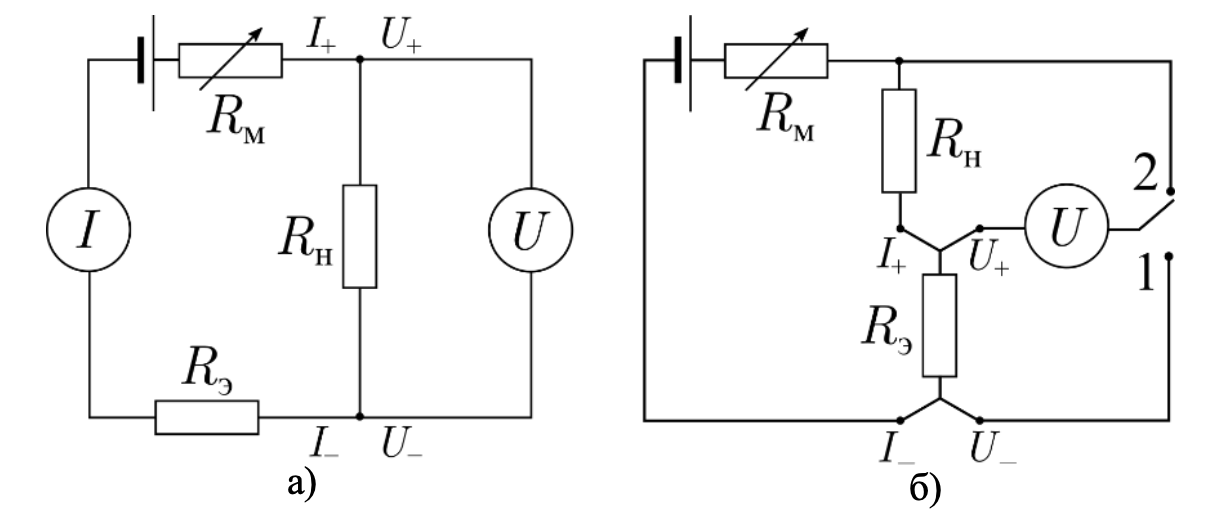
\includegraphics[scale = 0.5]{curcuit.png}
  \caption{Варианты электрических схем измерения сопротивления нити и мощности нагрева: а) с двумя мультиметрами, б) с одним вольтметром и эталонным сопротивлением}
  \label{fig:curcuit}
\end{figure}

В обеих схемах ток регулируется реостатом $R_\text{м}$, подключённым последовательно с источником питания.

\subsection*{Методика измерений}

Измерение сопротивления нити с током приводит к самонагреву:
\[
Q = I^2 R.
\]

Для исключения систематической ошибки используют метод экстраполяции: строится нагрузочная кривая $R(Q)$, и по её пересечению с осью $Q=0$ находят сопротивление $R_0$, соответствующее температуре окружающей среды $t_0$.

При этом можно аппроксимировать зависимость:
\[
R(t) = R_{273} \cdot (1 + \alpha t),
\]
где $R_{273}$ — сопротивление при $0^\circ$C, $\alpha$ — температурный коэффициент сопротивления:
\[
\alpha = \frac{1}{R_{273}} \frac{dR}{dt}.
\]

Измерения $R(Q)$ при разных $t_0$ дают $R(t)$. По наклонам кривых и формуле (\ref{}) определяется теплопроводность $\kappa$.

\section*{Ход работы}
\begin{center}
  \textsf{I. Подготовка к эксперименту}
\end{center}

\begin{enumerate}
    \item Проведём предварительные расчёты параметров опыта. Для этого зафиксируем параметры установки. 
    
    Нить платиновая. \\
    $R^{Pt}_0 \approx 20 \, \Omega$ — сопротивление нити при комнатной температуре; \\
    $2r_0 = (0.7 \pm 0.1) \, \text{см} = (7 \pm 1) \, \text{мм}$ — внутренний диаметр цилиндрической трубки; \\
    $2r_1 = (0.05 \pm 0.01) \, \text{мм}$ — диаметр платиновой нити; \\
    $L \approx 0.40 \, \text{м}$ — длина нити; \\
    $\Delta T = (30 \pm 1) \, K$ — максимальный перегрев нити относительно термостата при напряжении источника питания; \\
    $\kappa \approx 25 \frac{\text{мВт}}{\text{м}\cdot\text{K}} = 25 \cdot 10^{-3} \, \frac{\text{Вт}}{\text{м}\cdot\text{K}}$ — коэффициент теплопроводности воздуха (для оценки максимальной мощности нагрева). 
    
    Приняв максимально допустимый перегрев нити относительно термостата равным $\Delta t_{\text{max}} = 30^\circ$C, оценим максимальную мощность нагрева $Q_{\text{max}}$ [мВт] (см. формулу (\ref{Q})), которую следует подавать на нить. Для оценки примем коэффициент теплопроводности воздуха равным $\kappa \sim 25$ мВт/(м$\cdot$К).
    \[
      Q_{\text{max}} = \frac{2\pi L \kappa \Delta T}{\ln(r_0 / r_1)} = \frac{2 \pi \cdot 0.40 \cdot 25 \cdot 10^{-3} \cdot 30}{\ln(7/0.05)} = 0.381 \, \text{Вт}
    \]
\begin{itemize}
  \item По вычисленной мощности и приближенному значению сопротивления нити $R_\text{н}$ (см. техническое описание установки), определим соответствующие значения максимального тока $I_{\text{max}}$ и максимального напряжения $U_{\text{max}}$ на ней. 
  \[
    I_{\text{max}} = \sqrt{\frac{Q_{\text{max}}}{R_\text{н}}} \approx 138 \, \text{мА}
  \]
  \[
    U_{\text{max}} = \sqrt{Q_{\text{max}} R_\text{н}} \approx 2.76 \, \text{В}
  \]
  \item Перед переходом к измерениям покажем результаты расчёта преподавателю. При дальнейшей работе во избежание перегрева нити не допустим превышения данных параметров.
  \item Во избежание перегорания нити не увеличиваем напряжение на источнике питания $\mathcal{E}$ выше критического!
\end{itemize}

\item Подготовим экспериментальную установку.
\begin{itemize}
  \item Проверим, что измерительная цепь соответствует схеме рис. 3(а).
  \item На магазине сопротивлений установим такое сопротивление $R_m$, чтобы ток в цепи при её замыкании был минимален ($R_m \geqslant 90$ кОм).
  \item Включим вольтметр и амперметр и настроим режимы их работы.
  \item Включим источник питания; проверим, что он работает в режиме источника напряжения, и что напряжение на нём не превышает максимально допустимое ($U = 3.8$ В).
  \item Включим термостат и убедимся, что вода в нём находится при комнатной температуре $t = (23.0 \pm 0.1) ^\circ C$; при необходимости нагреем/охладим термостат.
\end{itemize}

\begin{center}
  \textsf{II. Проведение измерений}
\end{center}

    \item При фиксированной температуре термостата измерим зависимость сопротивления нити $R_n = \frac{U}{I}$ от подаваемой на неё мощности $Q = U I$ — нагрузочную кривую $R_n(Q)$.
    \[
      Q = UI = I^2 R_n = \frac{\mathcal{E}^2 R_n}{(R_n + R_m^2} 
    \]
    \[
      R_m = \mathcal{E} \sqrt{\frac{R_n}{Q_n}} - R_n
    \]

    \begin{itemize}
      \item Измерения проведём для 9–10 значений тока $I$ через нить от 0 до $I_{\text{max}}$.
      
      \item Постараемся подбирать такие значения сопротивления магазина $R_m$, чтобы мощность нагрева нити $Q = I^2 R_n$ возрастала приблизительно равномерно в диапазоне от 0 до $Q_{\text{max}}$.
      
      Во время работы мы воспользовались неправильной формулой и получили невразумительные результаты. Из-за чего напряжения подбирались на глаз, чтобы мощность возрастала примерно равномерно. И, разумеется, с ограничением по току, чтобы избежать перегорания нити.

      \begin{table}[h!]
        \centering
        \begin{tabular}{|c|cccccccccc|}
          \hline
          $Q$, мВт & 40 & 80 & 120 & 160 & 200 & 240 & 280 & 320 & 360 & 381 \\
          \hline
          $R_M$, $\Omega$ & 65 & 40 & 29 & 22 & 18 & 15 & 12 & 10 & 8.3 & 7.5 \\
          \hline
          \end{tabular}
        \label{tab:QRm}
        \caption{Значения сопротивлений магазина и предполагаемые мощности}
      \end{table}
    
      \item Ток следует наращивать монотонно, постепенно уменьшая сопротивление магазина сопротивлений $R_m$. Перед фиксацией показаний дождёмся установления теплового равновесия (время ожидания $\sim 30$ с): показания мультиметров должны быть стационарны (флуктуировать вблизи постоянного значения). 
      
      При измерениях будем не только записывать показания мультиметров (напряжение $U$ и ток $I$), но и сразу вычислять $R_n$ и $Q$. Погрелности $R_n$ и $Q$ рассчитаем по формуле $\varepsilon_Q = \varepsilon_{R_n} = \sqrt{\varepsilon_I^2 + \varepsilon_U^2}$.
      
      Результаты приведены в таблице Excel. Точек достаточно много, поэтому размещение их в отчете я считаю нецелесообразным. Вместо этого визуалируем данные на графике (\ref{fig:RQ}).
      
      \item В процессе измерений контролируем постоянство температуры термостата. Если за время измерений температура термостата изменилась более чем на 0,1℃, опыт будем переделывать. 
    \end{itemize}

    \item По окончании измерений нагрузочной кривой установим минимальный ток через нить, переведя значение магазина сопротивления на $R_m \geqslant 90$ кОм. В дальнейшем будем возвращать магазин сопротивлений в это положение после каждого измерения нагрузочной кривой.
    
    \item Проведём измерения нагрузочных кривых согласно п. 3–4 для 5–7 температур термостата в диапазоне от комнатной до 80℃ c интервалом в 10℃. Приступим к измерениям при новой температуре лишь после установления стационарного состояния (время ожидания не менее 15 минут).
    
    \item После завершения измерений выключим блок питания и цифровые мультиметры. На магазине сопротивлений (реостате) $R_m$ установим максимальное сопротивление ($\geqslant 90$ кОм). Поставим термостат на охлаждение до комнатной температуры.

\begin{center}
  \textsf{III. Обработка результатов измерений}
\end{center}

    \item Для каждой температуры термостата построим график зависимости сопротивления нити от мощности $R(Q)$. 
    
    Убедимся в линейности полученных зависимостей. Проведём наилучшие прямые методом МНК и определим точки их пересечения с осью ординат $R_0$ (при $Q \to 0$ температура нити совпадает с температурой термостата) и угловые коэффициенты наклона $\frac{dR}{dQ}$. 

    Для этого воспользуемся формулами.

    \[
      k = \frac{\langle xy \rangle - \langle x \rangle \langle y \rangle}{\langle x^2 \rangle - \langle x \rangle ^2} 
      = \frac{\langle QR \rangle - \langle Q \rangle \langle R \rangle}{\langle Q^2 \rangle - \langle Q \rangle ^2} 
    \]
    \[
      b = \langle y \rangle - k \langle x \rangle 
      = \langle R \rangle - k \langle Q \rangle 
    \]
    \[
      \sigma_k = \frac{1}{\sqrt{n}} \sqrt{\frac{\langle y^2 \rangle - \langle y \rangle ^2}{\langle x^2 \rangle - \langle x \rangle ^2} - k^2} 
      = \frac{1}{\sqrt{n}} \sqrt{\frac{\langle R^2 \rangle - \langle R \rangle ^2}{\langle Q^2 \rangle - \langle Q \rangle ^2} - k^2} 
    \]
    \[
      \sigma_b = \sigma_k \sqrt{\langle x^2 \rangle - \langle x \rangle ^2} 
      = \sigma_k \sqrt{\langle Q^2 \rangle - \langle Q \rangle ^2}
    \]

    Рассчитанные коэффициенты и их погрешности представлены в таблице (\ref{tab:ab}) и на графике (\ref{fig:RQ}), где $a$ соответствует угловому коэффициенту, а $b$ — свободному.

    \begin{figure}[h!]
      \centering
      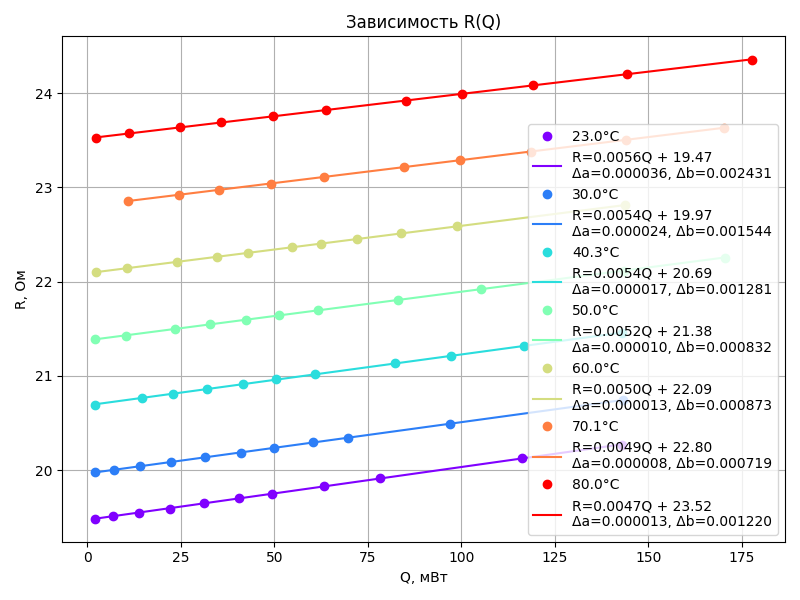
\includegraphics[scale = 0.75]{images/graph_RQ.png}
      \caption{Зависимость сопротивления нити от мощности}
      \label{fig:RQ}
    \end{figure}

    \begin{table}[h!]
      \centering
      \begin{tabular}{|c|c|c|c|c|c|}
        \hline
        $t,\,^{\circ}\text{C}$ & $R_0,\,\Omega$ & $\sigma_{R_0}\,\Omega$ & $\frac{dR}{dQ}, \, 10^{-5} \frac{\Omega}{\text{Вт}}$ & $\sigma_{\frac{dR}{dQ}}, \, 10^{-5} \frac{\Omega}{\text{Вт}}$ & $\varepsilon_{R_n} = \varepsilon_Q$ \\
        \hline
        23.0  & 19.4740 & 0.0024 & 560 & 3.6 & 0.008 \\
        30.0  & 19.9656 & 0.0015 & 545 & 2.4 & 0.008 \\
        40.3  & 20.6881 & 0.0013 & 539 & 1.7 & 0.008 \\
        50.0  & 21.3775 & 0.0008 & 515 & 1.0 & 0.008 \\
        60.0  & 22.0891 & 0.0009 & 503 & 1.3 & 0.008 \\
        70.1  & 22.8018 & 0.0007 & 487 & 0.8 & 0.008 \\
        80.0  & 23.5186 & 0.0012 & 472 & 1.3 & 0.008 \\
        \hline
      \end{tabular}
      \caption{Значения сопротивлений и коэффициентов нагрузочных прямых}
      \label{tab:ab}
    \end{table}

    \item Пользуясь значениями $R_0$ из таблицы (\ref{tab:ab}), построим график зависимости сопротивления нити от её температуры $R(T)$ (см. рисунок (\ref{fig:RT})). 
    
    \begin{figure}[h!]
      \centering
      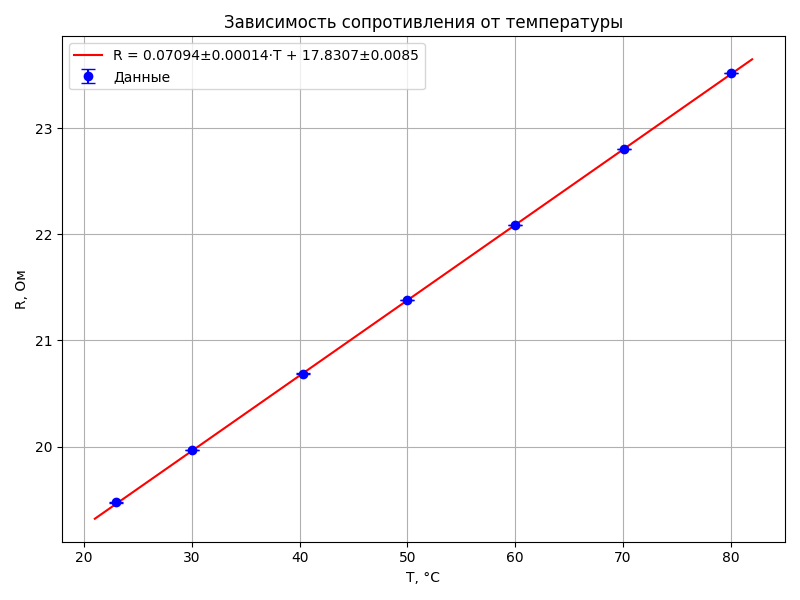
\includegraphics[scale=0.75]{graph_RT.png}
      \caption{Зависимость сопротивления от температуры}
      \label{fig:RT}
    \end{figure}

    Полученная зависимость линейна. Построим наилучшую прямую и определим её наклон $\frac{dR}{dT}$ с помощью метода наименьших квадратов. 

    \[
      k = \frac{\langle xy \rangle - \langle x \rangle \langle y \rangle}{\langle x^2 \rangle - \langle x \rangle ^2} 
      = \frac{\langle TR \rangle - \langle T \rangle \langle R \rangle}{\langle T^2 \rangle - \langle T \rangle ^2} 
      = 0.07094 \, \frac{{\Omega}}{^\circ C}
    \]
    \[
      b = \langle y \rangle - k \langle x \rangle 
      = \langle R \rangle - k \langle T \rangle = 17.8307 \, \Omega
    \]

    Оценим погрешности.
    \[
      \sigma_k = \frac{1}{\sqrt{n}} \sqrt{\frac{\langle y^2 \rangle - \langle y \rangle ^2}{\langle x^2 \rangle - \langle x \rangle ^2} - k^2} \frac{{\Omega}}{^\circ C}
      = \frac{1}{\sqrt{n}} \sqrt{\frac{\langle R^2 \rangle - \langle R \rangle ^2}{\langle T^2 \rangle - \langle T \rangle ^2} - k^2} 
      = 0.00014 \, \frac{{\Omega}}{^\circ C}
    \]
    \[
      \sigma_b = \sigma_k \sqrt{\langle x^2 \rangle - \langle x \rangle ^2} 
      = \sigma_k \sqrt{\langle T^2 \rangle - \langle T \rangle ^2} 
      = 0.0085 \,\Omega
    \]

    \[ 
      \frac{dR}{dT} = (0.07094 \pm 0.00014) \, \frac{{\Omega}}{^\circ C} = (7.094 \pm 0.014) \cdot 10^{-2} \, \frac{{\Omega}}{^\circ C}
    \]
    
    Сравним температурный коэффициент сопротивления материала нити $\alpha = \frac{1}{R_{273}} \frac{dR}{dT}$, где $R_{273}$ — сопротивление проволоки при $T = 273\, K$, с табличным.

    \[
      \alpha = \frac{1}{R_{273}} \frac{dR}{dT} = \frac{(7.094 \pm 0.014) \cdot 10^{-2} \, \frac{{\Omega}}{^\circ C}}{(17.831 \pm 0.009) \Omega} = (3.978 \pm 0.008) \cdot 10^{-3} \, \frac{1}{K}
    \]
    \[
      \alpha_{Pt} = (3.90 \pm 0.01) \cdot 10^{-3} \, \frac{1}{K}
    \]

    Значения отличаются на $2\%$.

    \item Используя угловой коэффициент температурной зависимости сопротивления п. 8 и угловые коэффициенты нагрузочных прямых из п. 7, вычислим наклон зависимости выделяющейся на нити мощности $Q$ от её перегрева $\Delta T$ относительно стенок для каждого из значений температур:
    \[
    \frac{dQ}{d(\Delta T)} = \frac{dR/dT}{dR/dQ}
    \]

    Рассчитанные значения приведены в таблице (\ref{tab:RDQ}).

    \begin{table}[h!]
      \begin{tabular}{|c|c|c|c|c|c|c|c|c|c|}
        \hline
        $t$, °C&$\frac{dR}{dQ}$, $\frac \Omega{\text{Вт}}$&$\frac{dQ}{d(\Delta T)}$, $\frac {\text{мВт}}{\text{К}}$&$\sigma\left({\frac{dQ}{d (\Delta T)}}\right)$, $\frac {\text{мВт}}{\text{К}}$&$k$, $\frac {\text{Вт}}{\text{м·К}}$&$\sigma_k$, $\frac {\text{Вт}}{\text{м·К}}$&$\ln T$&$\ln \frac{dQ}{d(\Delta T)}$&$\sigma_x$&$\sigma_y$\\ \hline
        23,0&5,60&12,67&0,07&0,0249&0,0014&5,6904&-4,369&0,0003&0,006\\ \hline
        30,0&5,438&13,04&0,06&0,0256&0,0014&5,7137&-4,340&0,0003&0,005\\ \hline
        40,3&5,394&13,15&0,05&0,0258&0,0014&5,7472&-4,332&0,0003&0,004\\ \hline
        50,0&5,153&13,76&0,04&0,0271&0,0015&5,7777&-4,2859&0,0003&0,0027\\ \hline
        60,0&5,026&14,11&0,04&0,0277&0,0015&5,8081&-4,261&0,0003&0,003\\ \hline
        70,1&4,874&14,55&0,04&0,0286&0,0016&5,8380&-4,2303&0,0003&0,0024\\ \hline
        80,0&4,720&15,02&0,05&0,0295&0,0016&5,8665&-4,198&0,0003&0,003\\ \hline
      \end{tabular}
      \caption{Расчет коэффициентов теплопроводности и $dQ/d(\Delta T)$}
      \label{tab:RDQ}
    \end{table}

    Отсюда, с учётом формулы (\ref{Q}), найдём коэффициенты теплопроводности газа $\kappa$ для каждой температуры термостата $T_0$. 
    \[
      Q = \frac{2\pi L \kappa \Delta T}{\ln(r_0 / r_1)}, \qquad \kappa = \frac{Q \ln(r_0 / r_1)}{2\pi L \Delta T}
    \]
    

    Оценим погрешности полученных результатов. 
    \[
      \varepsilon\left({\frac{dQ}{d (\Delta T)}}\right) = \sqrt{\varepsilon_Q^2 + \varepsilon_T^2 + 2\varepsilon_{R_0}^2 + {\varepsilon^\text{случ}_{dR/dT}}^2 + {\varepsilon^\text{случ}_{dR/dQ}}^2}
    \]
    \[
      \varepsilon_{\kappa} = \sqrt{\varepsilon_L^2 + {\varepsilon^\text{случ}_{dQ/dT}}^2 + \frac{\varepsilon_{r_0}^2 + \varepsilon_{r_1}^2}{\ln^2(r_0/r_1)}}
    \]
    
    Значения занесем в таблицу (\ref{tab:RDQ}).

    График зависимости $\kappa (T)$ изображен на рисунке (\ref{fig:kT}).

    \begin{figure}[h!]
      \centering
      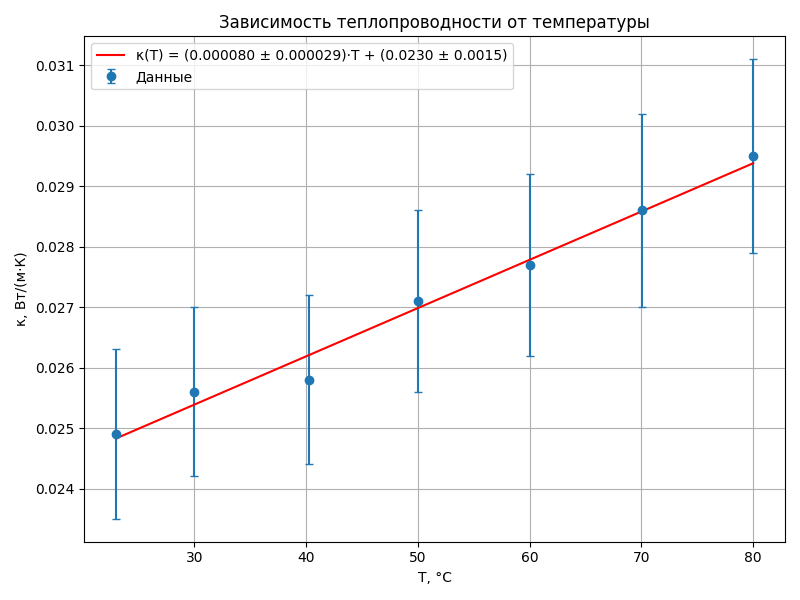
\includegraphics[scale=0.75]{graph_kT.png}
      \caption{Зависимость $\kappa (T)$}
      \label{fig:kT}
    \end{figure}

    \item Построим график зависимости теплопроводности воздуха от температуры газа $\kappa(T)$. Сравним результаты с табличными данными.
    
    Предполагая, что $\kappa$ степенным образом зависит от абсолютной температуры $T$: 
    \[
    \kappa \propto T^\beta,
    \]
    построим график в двойном логарифмическом масштабе (в координатах $\ln \kappa$ против $\ln T$) и определим из него показатель степени $\beta$. 
    
    В связи с тем, что значения $\kappa$ и $\frac{dQ}{d(\Delta T)}$ отличаются в $\frac{2 \pi L}{ln(r_0/r_1)}$ раз, графики $\ln \kappa$ от $\ln T$ и $\ln\frac{dQ}{d(\Delta T)}$ от $\ln T$ будут отличаться только смещением вдоль оси — коэффициент наклона останется неизменным.

    Рассчитаем погрешности. 
    \[
      \sigma_{\ln(dQ/d(\Delta T))} = \varepsilon_{dQ/d(\Delta T)}
    \]
    \[
      \sigma_{\ln T} = \varepsilon_{T}
    \]

    Значения занесем в таблицу (\ref{tab:RDQ}). График представлен на рисунке (\ref{fig:ln}), аппроксимирующая прямая проведена методом хи-квадрат.

    Рассчитаем погрешности.
    \[
      \sigma^{\text{случ}}_{\beta} = \sqrt{\frac{\langle x^2 \rangle - \langle x \rangle^2}{\sum_{i=1}^7 \frac{1}{\sigma_{y_i}^2}}}  = 0.025  
    \]
    \[
      \varepsilon^{\text{приб}}_{\beta} = \sqrt{\overline{\varepsilon^2_{x_i}} + \overline{\varepsilon^2_{y_i}}} \ll \varepsilon^{\text{случ}}_{\beta}
    \]

    Запишем значение $\beta$.
    \[
      \beta = (0.980 \pm 0.025) = (9.80 \pm 0.25) \cdot 10^{-1} 
    \]

    \begin{figure}[h!]
      \centering
      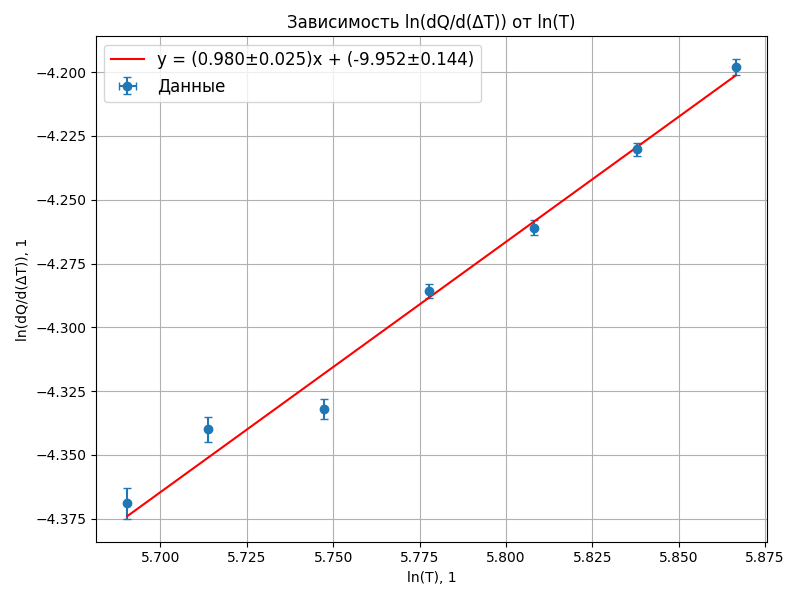
\includegraphics[scale=0.75]{graph_ln.png}
      \caption{Зависимость $\ln(\frac{dQ}{d(\Delta T)})$ от $\ln(T)$}
      \label{fig:ln}
    \end{figure}

    Проверим гипотезу о линейности. Больше 2/3 точек в пределах погрешности лежат на аппроксимирующей прямой (5 из 7).

    Число степеней свободы: \( \text{dof} = 7 - 2 = 5 \).

    \[
      \chi^2 = \sum_{i=1}^7 \frac{(y_i - a - b x_i)^2}{\sigma_{y_i}^2} = 23.5.
    \]  
    \[
      \chi^2/\text{dof} = 4.7
    \]

    Чтобы проверить гипотезу о линейности, нужно сравнить значение $\chi^2/\text{dof}$ с единицей. Значение \( \chi^2/\text{dof} = 4.7 \gg 1 \) указывает на отклонение от линейности или занижение погрешностей.  

    Полученное значение показателя степени $\beta$ вдвое превышает предсказанное упрощенной теорией ($\approx 1/2$), что заставляет предположить существование температурной зависимости эффективного сечения столкновений молекул.
\end{enumerate}

\section*{Вывод}

Все цели работы были достигнуты.

Зависимость коэффициента теплопроводности воздуха при атмосферном давлении от температуры измерена. Эта зависимость и промежуточные выводы указаны выше.

\end{document}

\begin{comment}
\section*{Ход работы}
\begin{center}
  \textsf{I. Подготовка к эксперименту}
\end{center}

\begin{enumerate}
    \item Проведём расчёты параметров опыта.
    \begin{itemize}
      \item Примем перегрев нити $\Delta t_{\text{max}} = 30^\circ$C и оценим максимальную мощность $Q_{\text{max}}$.
      \item Оценим максимальный ток $I_{\text{max}}$ и напряжение $U_{\text{max}}$ по значению сопротивления нити $R_n$.
      \item Покажем результаты расчёта преподавателю.
    \end{itemize}
  
    ВНИМАНИЕ! Не увеличим напряжение выше допустимого значения!

\item Подготовим экспериментальную установку.
\begin{itemize}
  \item Проверим схему подключения и установим сопротивление на магазине $R_m$ на 10 кОм.
  \item Настроим вольтметр и амперметр согласно техническому описанию.
  \item Включим источник питания и термостат, проверим температуру в термостате.
\end{itemize}

\begin{center}
  \textsf{II. Проведение измерений}
\end{center}

    \item Измерим зависимость сопротивления нити $R_n = \frac{U}{I}$ от мощности $Q = U I$ для 9–10 значений тока $I$.
    \begin{itemize}
      \item Регулярно наращиваем ток и уменьшаем сопротивление $R_m$.
      \item Проверим стабилизацию показаний мультиметров перед записью.
      \item Контролируем стабильность температуры термостата.
    \end{itemize}

    \item По завершении измерений установим минимальный ток через нить и вернём сопротивление $R_m$ на 10 кОм.
    \item Повторим измерения для 5–7 температур термостата.
    \item Выключим блок питания и мультиметры по завершении работы, установим максимальное сопротивление на $R_m$.
    
\begin{center}
  \textsf{III. Обработка результатов}
\end{center}

    \item Построим график зависимости $R(Q)$ для каждой температуры, оценим линейность, найдем $R_0$ и $\frac{dR}{dQ}$.
    \item Построим график зависимости $R(T)$ и определим наклон $\frac{dR}{dT}$.
    \item Вычислим наклон зависимости $Q(\Delta T)$ и определим коэффициент теплопроводности $\kappa$ для разных температур.
    \item Построим график зависимости $\kappa(T)$ и определим показатель степени $\beta$.
\end{enumerate}
\end{comment}